% Conics: The projective construction of polars and  tangents
% Author: Hugues Vermeiren
\documentclass{standalone}
\usepackage{tikz}
\usetikzlibrary{calc,intersections}

\begin{document}
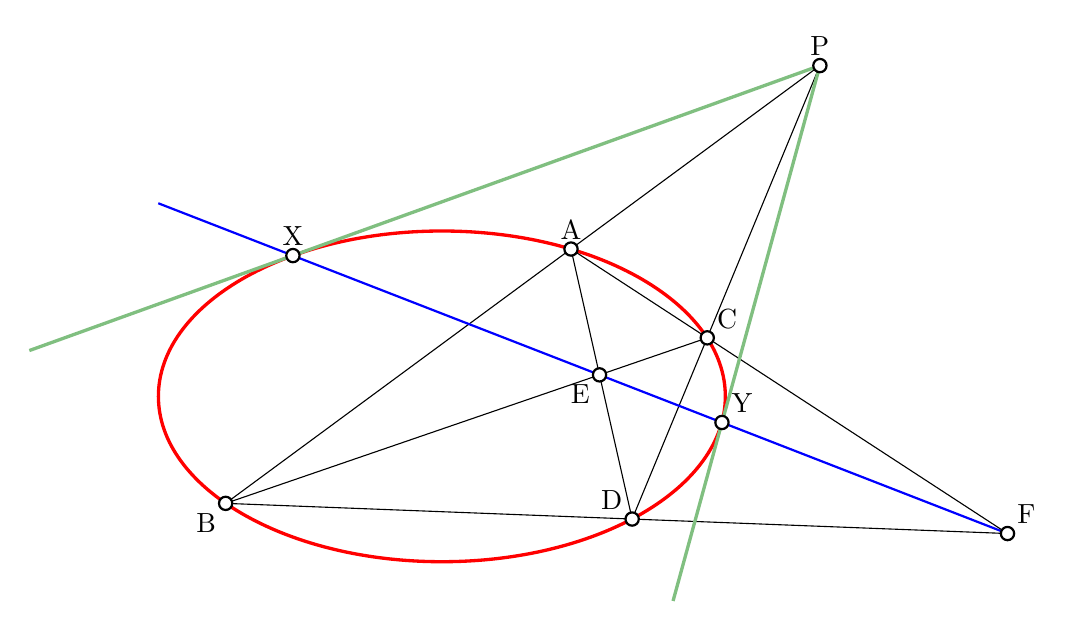
\begin{tikzpicture}[scale=1.2]
	\tikzset{mypoints/.style={fill=white,draw=black,thick}}
	\def\ptsize{2.0pt}
	\def\a{3} \def\b{1.75}
	% warning: construction fails if xp<0 or yp<=0
	\def\xp{4.0} \def\yp{3.5} 
	\def\i{0.85} \def\j{-0.25}%determines rays from P
	\coordinate[label=above:P] (P) at (\xp,\yp);
	\coordinate (M) at ({\a*\i},0);
	\coordinate (N) at ({\a*\j},0);
	\coordinate (AA) at (0,-\b);
	\coordinate (BB) at (1,-\b);
	\coordinate (CC) at (-\a,0);
	\coordinate (DD) at (-\a,1);
	\coordinate (Q) at (intersection of P--N and AA--BB);
	\coordinate (R) at (intersection of P--M and AA--BB);
	\draw[name path=ellipse,red,very thick]
	(0,0) circle[x radius = \a cm, y radius = \b cm];
	\path[name path=linePQ,blue] (P)--(Q);
	\path[name path=linePR,green] (P)--(R);
	\path [name intersections={of = ellipse and linePQ}];
	\coordinate[label=above:A] (A)  at (intersection-1);
	\coordinate[label=below left:B] (B) at (intersection-2);
	\path [name intersections={of = ellipse and linePR}];
	\coordinate[label=above right:C] (C)  at (intersection-1);
	\coordinate[label=above left:D] (D) at (intersection-2);
	\draw (B)--(P)--(D) (A)--(D) (C)--(B);
	\coordinate [label=below left:E] (E) at (intersection of A--D and B--C);
	\coordinate[label=above right:F] (F) at (intersection of A--C and B--D);
	\coordinate (G) at (intersection of E--F and CC--DD);
	\draw [name path=lineFG,blue,thick] (F)--(G);
	\draw (A)--(F)--(B);
	\path [name intersections={of = ellipse and lineFG}];
	\coordinate[label=above:X] (X) at (intersection-1);
	\coordinate[label=above right:Y] (Y) at (intersection-2);
	\coordinate (XX) at ($(P)!1.5!(X)$);
	\coordinate (YY) at ($(P)!1.5!(Y)$);
	\draw[very thick,green!50!black!50] (XX)--(P)--(YY);
	\foreach \p in {A,B,C,D,E,F,P,X,Y}
	\fill[mypoints] (\p) circle (\ptsize);
\end{tikzpicture}
\end{document}